% !TEX root = ../../SPP_IoTjournal.tex
\subsection{Effect of Disturbance and Scheduled Time of Arrival \label{sec:city_distbEffect}}
In this section, we illustrate how the disturbance bound $d_r$ in \eqref{eq:dyn_i} and the realtive $\sta$s of vehicles affect the vehicle trajectories. For this purpose, we simulate the SPP algorithm for four additional scenarios:
\begin{itemize}
\item Case-0: $d_r = 6m/s$, $\sta_i = 0 ~\forall i$
\item Case-1: $d_r = 11m/s$, $\sta_i = 0 ~\forall i$
\item Case-2: $d_r = 6m/s$, $\sta_i = 5(i-1) ~\forall i$
\item Case-3: $d_r = 11m/s$, $\sta_i = 5(i-1) ~\forall i$
\item Case-4: $d_r = 11m/s$, $\sta_i = 10(i-1) ~\forall i$
\end{itemize}
The interpretation $\sta_i = 5(i-1)$ is that the scheduled time of arrival of any two consecutive vehicles is separated by 5s. $d_r = 6m/s$ and $d_r = 11m/s$ correspond to the moderate winds and strong winds respectively on Beaufort wind force scale \cite{Windscale}. 

Intuitively, as $d_r$ increases, it is harder for a vehicle to closely track a particular nominal trajectory, which results in a higher tracking error bound. \SBnote{Add the exact error bounds here.} Thus, the vehicles need to be separated more from each other in space to ensure that they do not enter each other's danger zones. This is also evident from comparing the results corresponding to Case-0 (Fig. \ref{fig:sf_d6sep0}) and Case-1 (Fig. \ref{fig:sf_d11sep0}). As the disturbance magnitude increases from $d_r = 6m/s$ (moderate winds) to $d_r = 11m/s$ (strong winds), the vehicles' trajectories get farther apart from each other. Since $\sta$ is same for all vehicles, the vehicles’ trajectories are still predominately \textit{state-separated} trajectories.

We next compare Case-0 and Case-2. The difference between these two cases is that vehicles have different $\sta$s in Case-2. When vehicles $\veh_i$ and $\veh_{j}$ ($j>i$) have same scheduled time of arrival and are going to the same destination, they are constrained to travel at the same time to make sure they reach the destination by the designtaed $\sta$. However, since $\veh_i$ is high-priority, it gets access to the optimal trajectory (in terms of the total time of tarvel to destination) and $\veh_{j}$ has to settle for a relatively sub-optimal trajectory. Thus, all vehicles going to a particular destination take different trajectories creating a ``band" of trajectories between the origin and the destination, as shown in Figure \ref{fig:sf_d6sep0}; the high-priority vehicles take a relatively straight path between the origin and the destination whereas the low-priority vehicles take a (relatively sub-optimal) curved path. If we think of an air highway between the origin and the destination, then vehicles take different lanes of that highway to reach the destination in Case-0. Thus, the trajectories of vehicles in this case are \textit{state-separated}. However, when $\sta_j > \sta_i$, then $\veh_j$ is not bound to travel at the same time as $\veh_i$; it can wait for $\veh_i$ to depart and take a shorter path later on. Thus, vehicles travel in a single (optimal) lane in this case, as shown in Figure \ref{fig:sf_d6sep5}. In other words, they take the same trajectory to the destination, but at different times. Thus, the trajectories of vehicles in this case are \textit{time-separated}. 

Note that the exact number of lanes depends on both the disturbance and relative $\sta$s. As disturbance increases, the vehicles need to be separated more from each other to ensure safety. The relative difference in $\sta$s should be able to ensure this separation if they were to take the same lane. As shown in Figure \ref{fig:sf_d11sep5}, a difference of 5s in $\sta$s is not sufficient to achieve a single lane behavior for strong winds. However, the number of lanes are significantly less than that in Case-1 (Fig. \ref{fig:sf_d11sep0}). Finally, a difference of 10s in $\sta$s ensure that we get the single lane behavior even in the presence of strong winds, leading to \textit{time-separated} trajectories. \SBnote{Add link to the simulation videos for each result.}

Overall, the relative magnitude of disturbance and scheduled times of arrival separation determines the number of lanes and type of trajectories that emerge out of the SPP algorithm. For a fixed disturbance magnitude, as the relative separation in the scheduled times of arrival of vehicles increases, the number of lanes between a pair of origin and destination decreases, and more and more tarjectories become time-separated. On the other hand, for a fixed relative separation in the scheduled times of arrival of vehicles, as the disturbnace magnitude increases, the number of lanes between a pair of origin and destination increases, and more and more tarjectories become state-separated.
%
\begin{figure*}[!htb]
 \centering
\begin{subfigure}{0.5\columnwidth}
  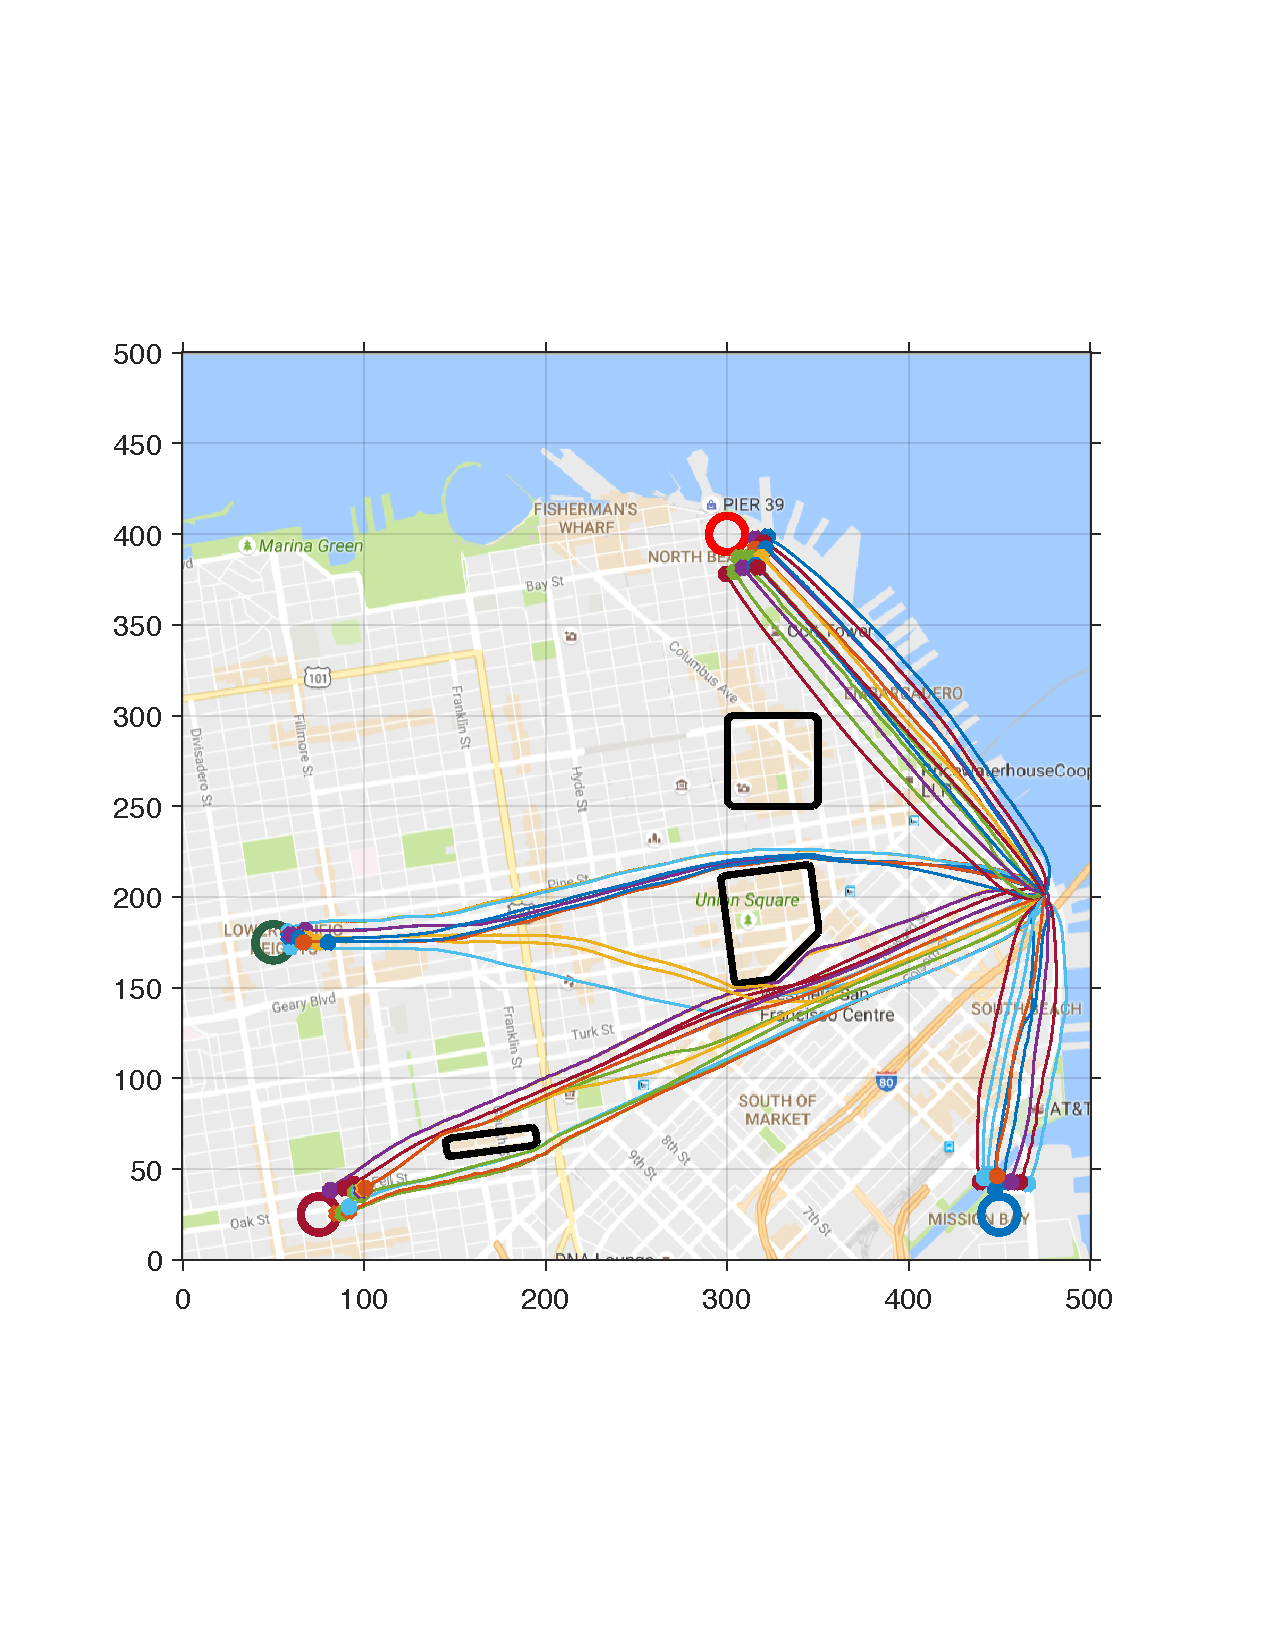
\includegraphics[width=\columnwidth]{figs/sf_d6sep0}
  \subcaption{Case-0: $d_r = 6m/s$, $\sta_i = 0$}
  \label{fig:sf_d6sep0}
\end{subfigure}%
\begin{subfigure}{0.5\columnwidth}
  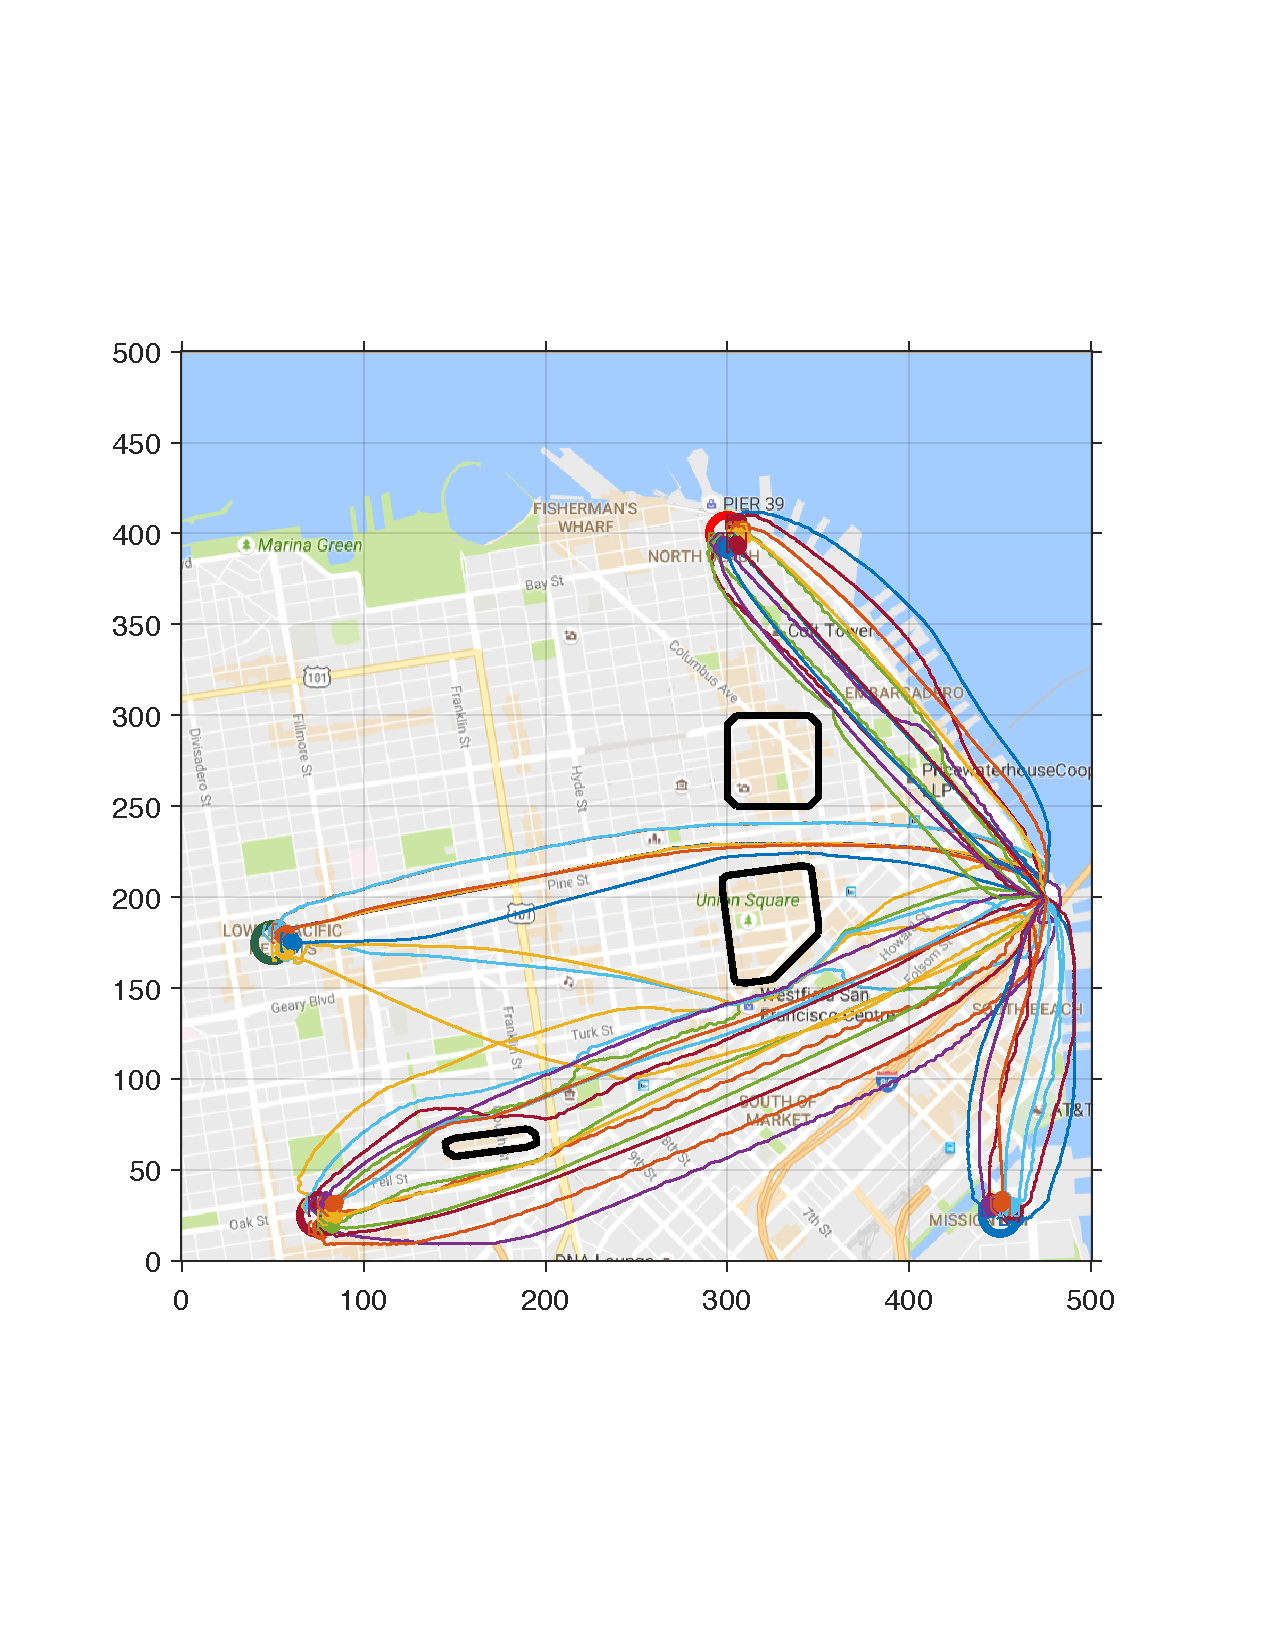
\includegraphics[width=\columnwidth]{figs/sf_d11sep0}
  \subcaption{Case-1: $d_r = 11m/s$, $\sta_i = 0$}
  \label{fig:sf_d11sep0}
\end{subfigure}%

\begin{subfigure}{0.5\columnwidth}
  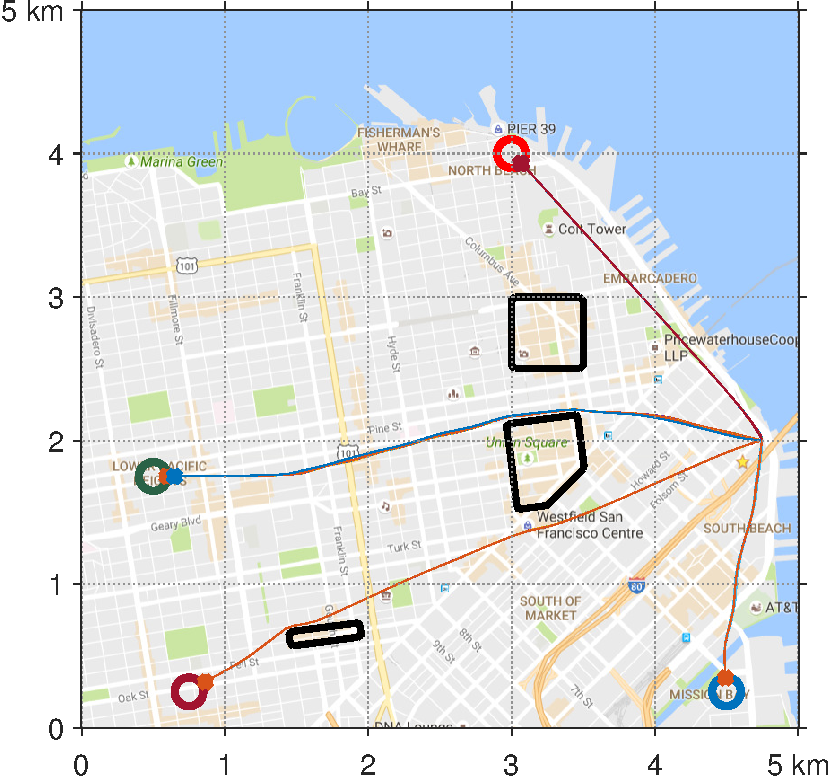
\includegraphics[width=\columnwidth]{figs/sf_d6sep5}
  \subcaption{Case-2: $d_r = 6m/s$, $\sta_i = 5(i-1)$}
  \label{fig:sf_d6sep5}
\end{subfigure}%
\begin{subfigure}{0.5\columnwidth}
  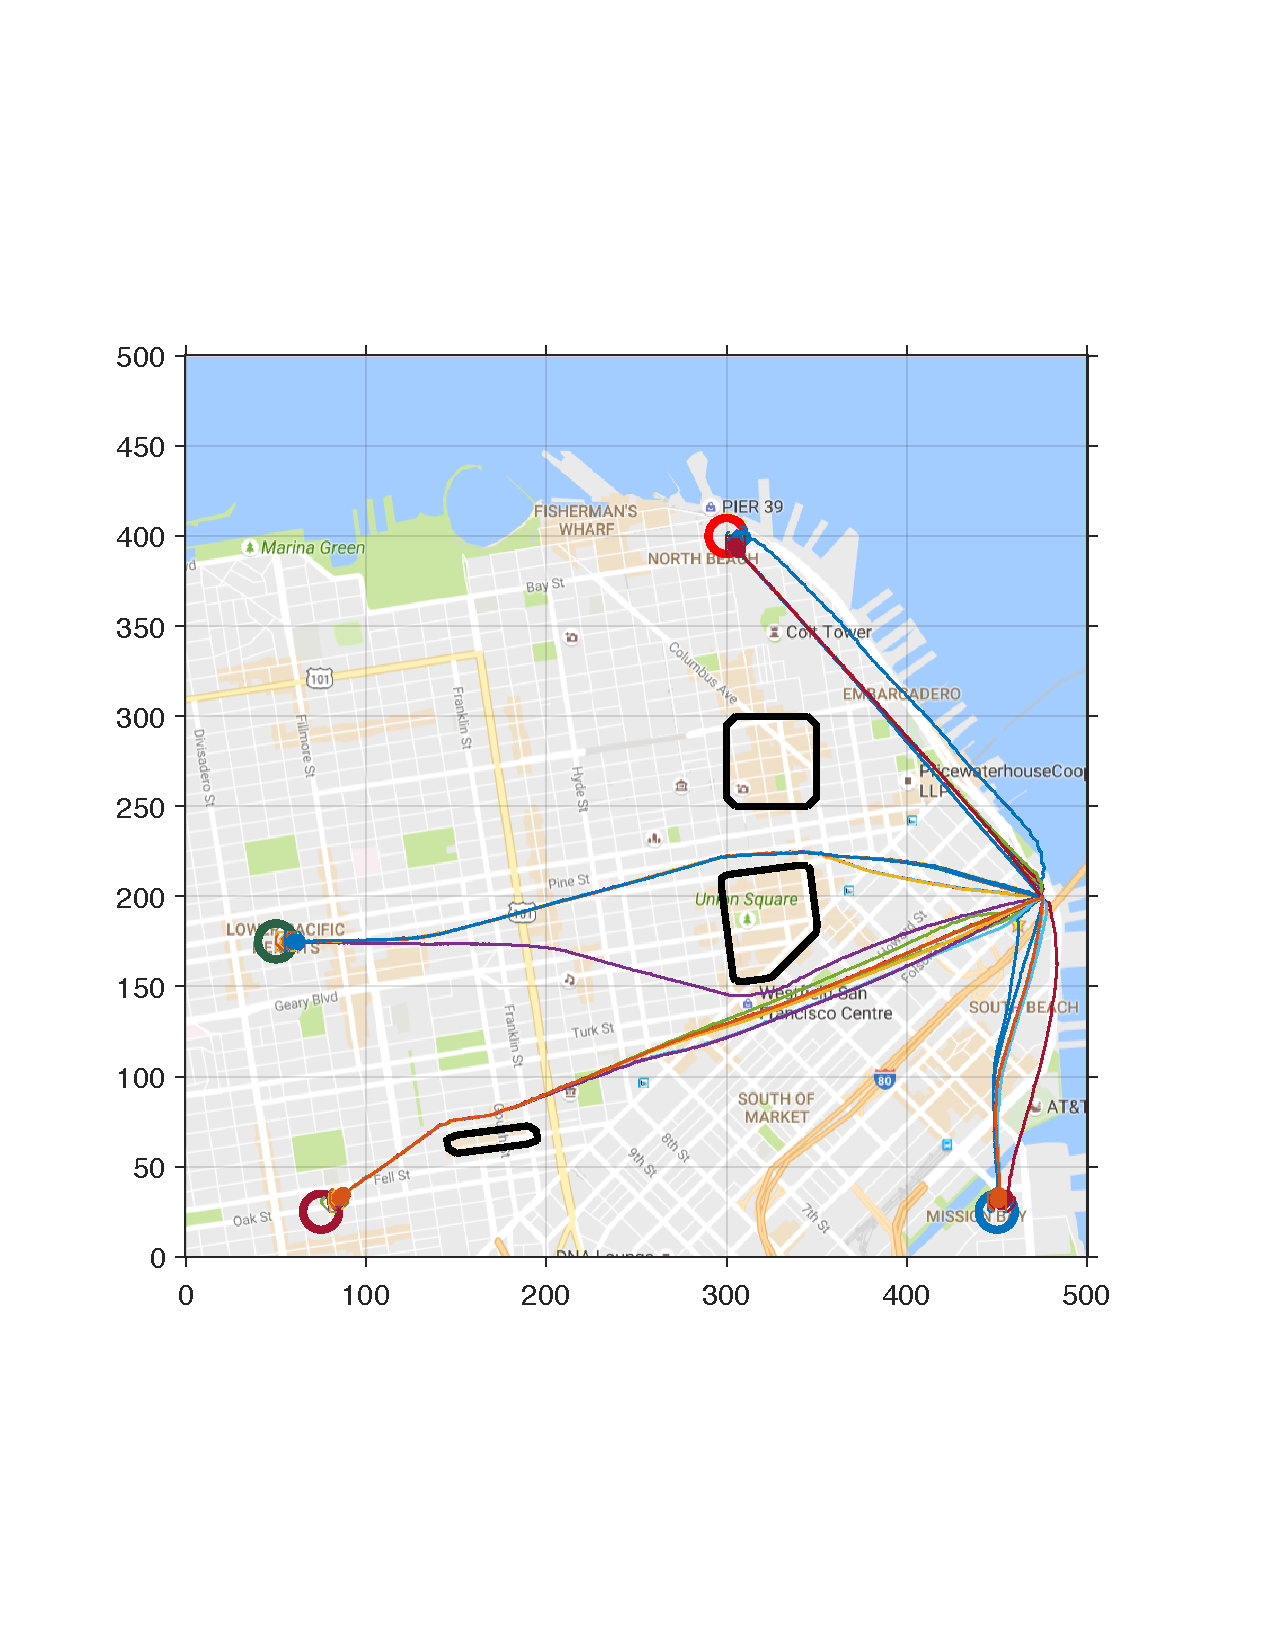
\includegraphics[width=\columnwidth]{figs/sf_d11sep5}
  \subcaption{Case-3: $d_r = 11m/s$, $\sta_i = 5(i-1)$}
  \label{fig:sf_d11sep5}
\end{subfigure}%
\caption{Effect of the disturbance magnitude and the scheduled times of arrival on vehicle trajectories. All trajectories are simulated under uniformly random disturbance. The relative separation in the scheduled times of arrival of vehicles determines the number of lanes between a pair of origin and destination, and more and more tarjectories become time-separated as this relative separation increases. The disturbnace magnitude determines the relative separation between different lanes, and more and more tarjectories become state-separated as the disturbance increases. }
\label{fig:trajectories_sf}
\end{figure*}

\begin{figure}[t]
  \centering
  \includegraphics[width=\columnwidth]{"figs/sf_d11sep10"}
  \caption{Vehicle trajectories for Case-4: $d_r = 11m/s$, $\sta_i = 10(i-1)$. Since different vehicles have different scheduled times of arrival, there is a single lane between every origin-destination pair.} 
  \label{fig:sf_d11sep10}
\end{figure}